% !TEX root = illustrator_submission.tex

\section{CMYK Support}
\label{sec:cmyk}

\Illustrator/ artwork is typically authored in the CMYK color space---optionally with spot color components---to
best facilitate high-quality color printing.
\Illustrator/ uses \AGM/ to render CMYK documents to a true CMYK framebuffer.
This means the color components in the rendered framebuffer
correspond to actual CMYK process colors plus any spot colors so blending and other color math
operates on and maintains the components independently.

What the artists sees ``on screen'' when editing a CMYK document is a color conversion from CMYK plus any spot colors
to RGB.  Importantly this conversion happens on the {\em final} CMYK rendering result; the conversion may even emulate the
specific color profile of a particular print device using ACE.
Converting CMYK rendering results to a print device's CMYK
color profile results in better color fidelity and gives an artist better access to the printer's full color gamut
including spot color inks.  Importantly spot color components stay segregated from process colors.

While it is possible to force the conversion of all CMYK color inputs to RGB and render in the GPU's conventional
RGB mode, Figure~\ref{fig:cmyk-vs-rgb-emulation} shows
the inadequacy of rendering CMYK content with this approach; notice the obvious color shifts.

\begin{figure}[tb]
  \center{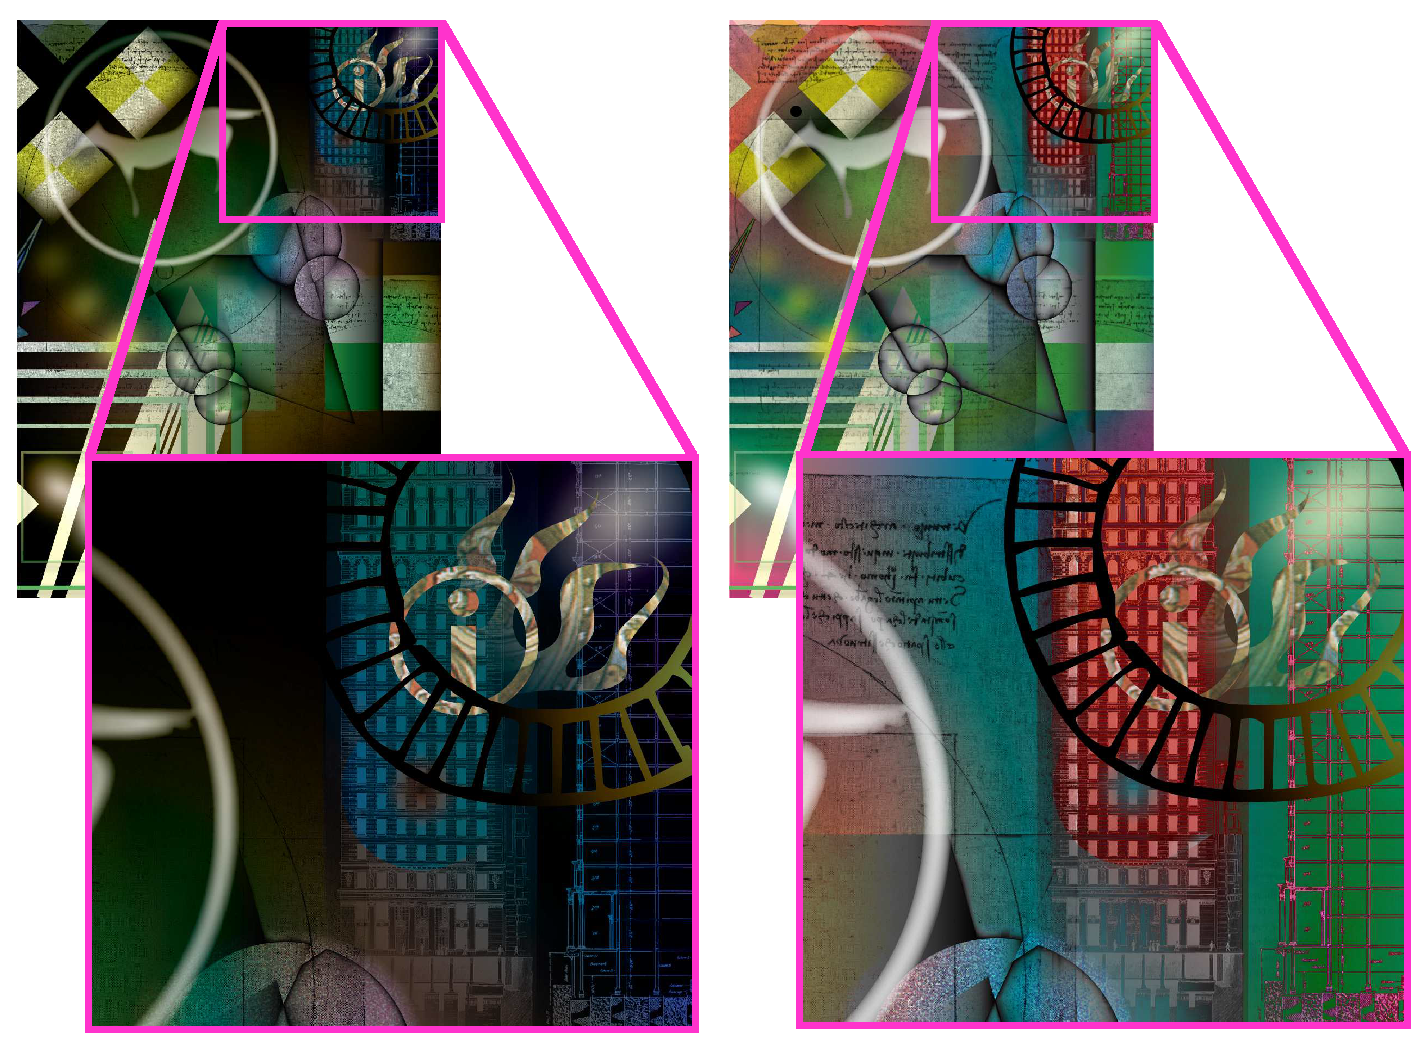
\includegraphics[width=3.3in]{images/cmyk_vs_rgb_emulation.pdf}}
  \caption{\label{fig:cmyk-vs-rgb-emulation} An artistic CMYK \Illustrator/ document (left, correct) properly rendered
in its intended CMYK color space; na\"{\i}ve RGB rendering (right-side, wrong) of same scene by converting all inputs to RGB .  Magnified portion show obvious gross color shifts.}
\end{figure}

Now we explain our approach to orchestrate CMYK rendering with multiple RGBA color buffers.
The technique we present works not just for \Illustrator/ but any GPU application that requires
CMYK rendering semantics.

There are two problems we must address:
\begin{enumerate}
\item CMYK is a subtractive color space so conventional GPU blending modes do not blend appropriately for CMYK.
\item At a minimum, CMYK rendering needs 5 framebuffer components---plus additional components for any spot colors.
\end{enumerate}

\subsection{CMYK Blend Modes and Color Math}
\label{sec:cmykblend}

Adobe's technical note introducing transparency to PDF \cite{TransparencyInPDF} explains how blending
in a subtractive color space requires special handling:
\begin{quote}
\small
When performing blending
operations in subtractive color spaces, we assume that the color component values are complemented before the blend mode function is applied and that the results of the function are then complemented before being used. By
complemented we mean that a color component value $c$ is replaced with $1 - c$. 
\end{quote}
An example helps appreciate why:  Consider a black ink at 90\% of its full application (so a dark black).  Now
consider how to get 40\% of the apparent brightness of that ink.  Intuitively 40\% brightness should be an
even darker black.
Na\"{\i}vely multiplying 0.9 by 0.4, as appropriate for additive color
components, is 36\% but less black ink is clearly incorrect.
Adjusting the blending math for the subtractive nature of black ink,
$1-((1-0.9)\times(1-0.4))$ = 94\% results in more black ink and the darker black we intuitively expect.

\begin{figure}[tb]
  \center{\includegraphics[width=2.9in]{images/rgba_vs_cmyk_blending.pdf}}
  \caption{\label{fig:rgba-vs-cmyk-blending} RGBA blending works normally (left); CMYK's subtractive color space must complement colors components on input and output of blending (right).}
\end{figure}

Figure~\ref{fig:rgba-vs-cmyk-blending} illustrates how RGB and CMYK
color values must be treated for a blend mode to operate correctly.
Conventional fixed-function GPU blending lacks the ability to complement
inputs and outputs to fixed-function blending.

The blend mode extensions described in Section~\ref{sec:blendmodes}
assume an additive color space.  Na\"{i}vely
adapting these blend modes to operate
correctly for a subtractive color space such as CMYK would mean adding
a complement to each input color component and, likewise, a complement
to each output color component.  We avoid the na\"{i}ve approach because
\begin{enumerate}

\item Additive blend modes avoid input \& output color component
complements so involve fewer operation
and are therefore more efficient.

This is particularly important for legacy hardware that predates
hardware blend mode support.
For such hardware, performing additional input \& output complements for
CMYK rendering would force expensive shader emulation
even for the default {\em Normal} blend mode that otherwise
can be performed with fast standard hardware blending.

\item Not just blending math
requires this adjustment---{\em all} color math such as in a shader or texture filtering must follow the rule.

\end{enumerate}
Our solution stores CMYK color components always in complemented form on the GPU.
Figure~\ref{fig:cmyk-gpu-blending} illustrates this approach.  Incoming CMYK colors, no matter what the source, must be
complemented.  Alpha values are {\em not} complemented and simply stored normally as alpha is always additive.

\begin{figure}[tb]
  \center{\includegraphics[width=\columnwidth]{images/cmyk_gpu_blending.pdf}}
  \caption{\label{fig:cmyk-gpu-blending} Conventional GPU blending works for CMYK when color components (but not alpha) are stored as complemented values.}
\end{figure}

The implications of this are far reaching and demand rigorous consistency.
Any CMYK or RGB color inputs must be converted to
complemented CMYK. 
For example, when color channels are logically ``cleared to zero,'' that really means clearing to one (but alpha
components still clear to zero).
By storing complemented CMYK colors in the framebuffer {\em and} in textures,
existing hardware texture accesses to such resources including texture filtering operate properly.
Likewise programmable
shaders are simpler and faster by skipping the requirement to complement input and output colors
by performing color math
on complemented subtractive color values.

Importantly our solution means the blend modes provided by the blend
equation advanced extensions operate in subtractive CMYK color mode
with exactly the same blending math as additive RGB color mode.

Only when rendered results are ready to be displayed or read back to
system memory should the complemented color components be reversed to uncomplemented CMYK.
Often color profiles are applied when displaying
or reading back rendering results so the necessary complement can be folded into a more complex conversion
thereby avoiding an explicit complement.  The bottom right two steps in Figure~\ref{fig:cmyk-gpu-blending} show this.

\subsection{Representing an NChannel Framebuffer on a GPU}
\label{sec:representing-cmyk}

When we speak of \Illustrator/'s CMYK color mode,
we mean a subtractive color spaces supporting the 4 standard print
process colors (CMYK), alpha, and possibly some fixed number of spot colors.  PDF supports
a variety of color spaces with different properties and degrees of sophistication.
The most general of these is the {\em NChannel}
color space so we use the term NChannel to refer to a general multi-component color space.

\subsubsection{Multiple Color Buffers}
\label{sec:multiplebuffers}

GPUs lack native support for color buffer configurations with more than 4 components.
However modern GPUs also support multiple (typically eight) color buffers to which a single
fragment shader can output a distinct RGBA value to each color buffer.  Each color buffer
is independently blended with its respective RGBA output value.

% UNINTERESTING
% Modern GPUs support {\em separate} fixed-function blend functions and equations
% on the RGB and A components of each 4-component RGBA color buffer.  The relevant point being that
% the fourth component, alpha, can be configured for blend math different than the other three (RGB).
% Indeed blend modes composite the alpha component different from the color components, hence
% this specialized behavior.

\begin{figure}[tb]
  \center{\includegraphics[width=3.3in]{images/cmyk_to_gpu_representation.pdf}}
  \caption{\label{fig:cmyk-to-rgba} How NChannel color components in a CMYK color space with spot colors are converted to a GPU-resident version.}
\end{figure}

We orchestrate multiple color buffers to ``construct'' an NChannel framebuffer with CMYKA components plus any
additional spot color components.
Figure~\ref{fig:cmyk-to-rgba} illustrates how we take a CMYKA input color with five spot color components
and convert this 10-component vector into a GPU-amenable representation by spanning three RGBA color buffers.
We can span additional color buffers to support more spot colors but we always require at least two
RGBA color buffers for CMYKA.

Figure~\ref{fig:cmyk-to-rgba} shows we {\em replicate} the alpha (A) component in the alpha of each RGBA color buffer.
This is done because blend mode equations for color values require access to the alpha component.  As GPU blending performs
each color buffer blending operation separately, replication of alpha ensures every three color components
of the NChannel color spanning multiple RGBA buffers has an accessible alpha value.  We deliberately replicate
alpha this way and ensure all alpha blending is identically configured so the alpha values of
each RGBA color buffer for any specific color sample maintain the {\em same} alpha value.
This invariant must be maintained for correct operation.

\subsubsection{Memory Requirements}
\label{sec:memory}

Our approach wastes some storage.
Every additional RGBA buffer adds an
additional replicated alpha component.  We also waste storage if the actual CMYK color mode configuration
has fewer spot colors than our multiple RGBA color buffers provide.  For example, CMYKA with zero spot
colors means the G and B components of the second color buffer are wasted---assuming R is used to store K.
The unfortunate implication is that a document in CMYK color mode without spot colors requires double
the framebuffer memory as an RGBA document.

This waste is substantial when coupled with \Illustrator/'s reliance on 8x multisampling for antialiasing.
When also accounting for the stencil buffer requirements, representing CMYK at 8x on today's GPUs requires 96 bytes
of storage per pixel.\footnote{96 bytes = $8 \times$ ( 4 bytes for depth-stencil + 8 bytes for CMYKA)}  
Each gigabyte of memory roughly corresponds to
representing 5.5 million CMYKA pixels this way.
The waste is ameliorated by the enormous memory capacity and bandwidth of modern GPUs.
Graphics boards with 12 gigabytes of memory are available today and capacities are sure to increase.

We anticipate GPU hardware innovations
will provide less wasteful memory organizations in future GPUs. In the interim
when the memory burden is just too taxing, settling for 4x antialiasing quality
easily halves the memory requirements at the cost of diminished rendering quality.

\subsubsection{Fragment Shader and Blending Implementation Details}
\label{sec:tweaks}

Once we have orchestrated multiple color buffers to store NChannel color values, our fragment shaders
must adapt to outputting color values appropriately.  This means making sure alpha is replicated in each
output color buffer alpha component and each process and spot color
is routed to its appropriate component in the correct color buffer.  

GPU color blending should be configured the same across all the framebuffer components.

One irksome detail:  The blend equation advanced extensions are restricted to operate only where outputting to the
first color buffer and requiring all other color buffers disabled (otherwise an OpenGL error is generated; this
reflects a hardware limitation).  We workaround this limitation with multiple ``cover'' steps.
We ``stencil'' the path once and then perform the path rendering ``cover''
operation repeatedly, once for each color buffer
(binding each color buffer in turn as the first and only color buffer)
and reset the stencil values only on the last color buffer.
Our fragment shader must be aware in this case which logical color buffer it is outputting in each repeated ``cover'' step.
While expensive, we only require this workaround for blend modes (typically the less common
ones) that do not correspond to fixed-function GPU blending---so importantly not the {\em Normal} mode.

\subsubsection{Reading an NChannel Framebuffer from a Shader}

\Illustrator/ occasionally needs to read a framebuffer from a shader.
(see Section~\ref{sec:non-isolated-groups} for an example).
To enable efficient texture lookup, we
organize the multiple color buffers
used to represent an NChannel
buffer
as layers
of a multisample 2D {\em texture array} ({\tt sampler2DMSArray} in GLSL
shaders).  A 2D texture array
is a single OpenGL texture object with a fixed format, width, height, and number of layers. 
When
multisampled, the number of samples is also fixed.
The {\tt texelFetch} command in a shader fetches an RGBA
floating-point vector sample from a given 2D location, layer index, and sample index (effectively a 4-dimensional array access).
Multiple {\tt texel\-Fetch} fetches, one to each layer, are necessary
from the fragment shader to read all the components of a pixel in an
NChannel framebuffer.

The \ARBtms/ extension \cite{TextureMultisample} introduced support for
multisampled 2D texture arrays with OpenGL 3.2 mandating the functionality.
Among the advantages of a multisampled 2D texture array is all the layers belong to a single texture memory allocation
making the layers faster to bind as a unit and managed as a single large memory allocation.
The OpenGL command {\tt glFramebuffer\-Texture\-Layer} allows
each layer of the texture array to be attached to different color buffer
of single framebuffer object.
